\documentclass[border=10pt]{standalone}

\usepackage{tikz}
\usepackage{tikzsymbols}
\usetikzlibrary{calc,patterns,shapes.geometric}

\def\centerarc[#1](#2)(#3:#4:#5){\draw[#1] ($(#2)+({#5*cos(#3)},{#5*sin(#3)})$) arc (#3:#4:#5);}

\begin{document}
	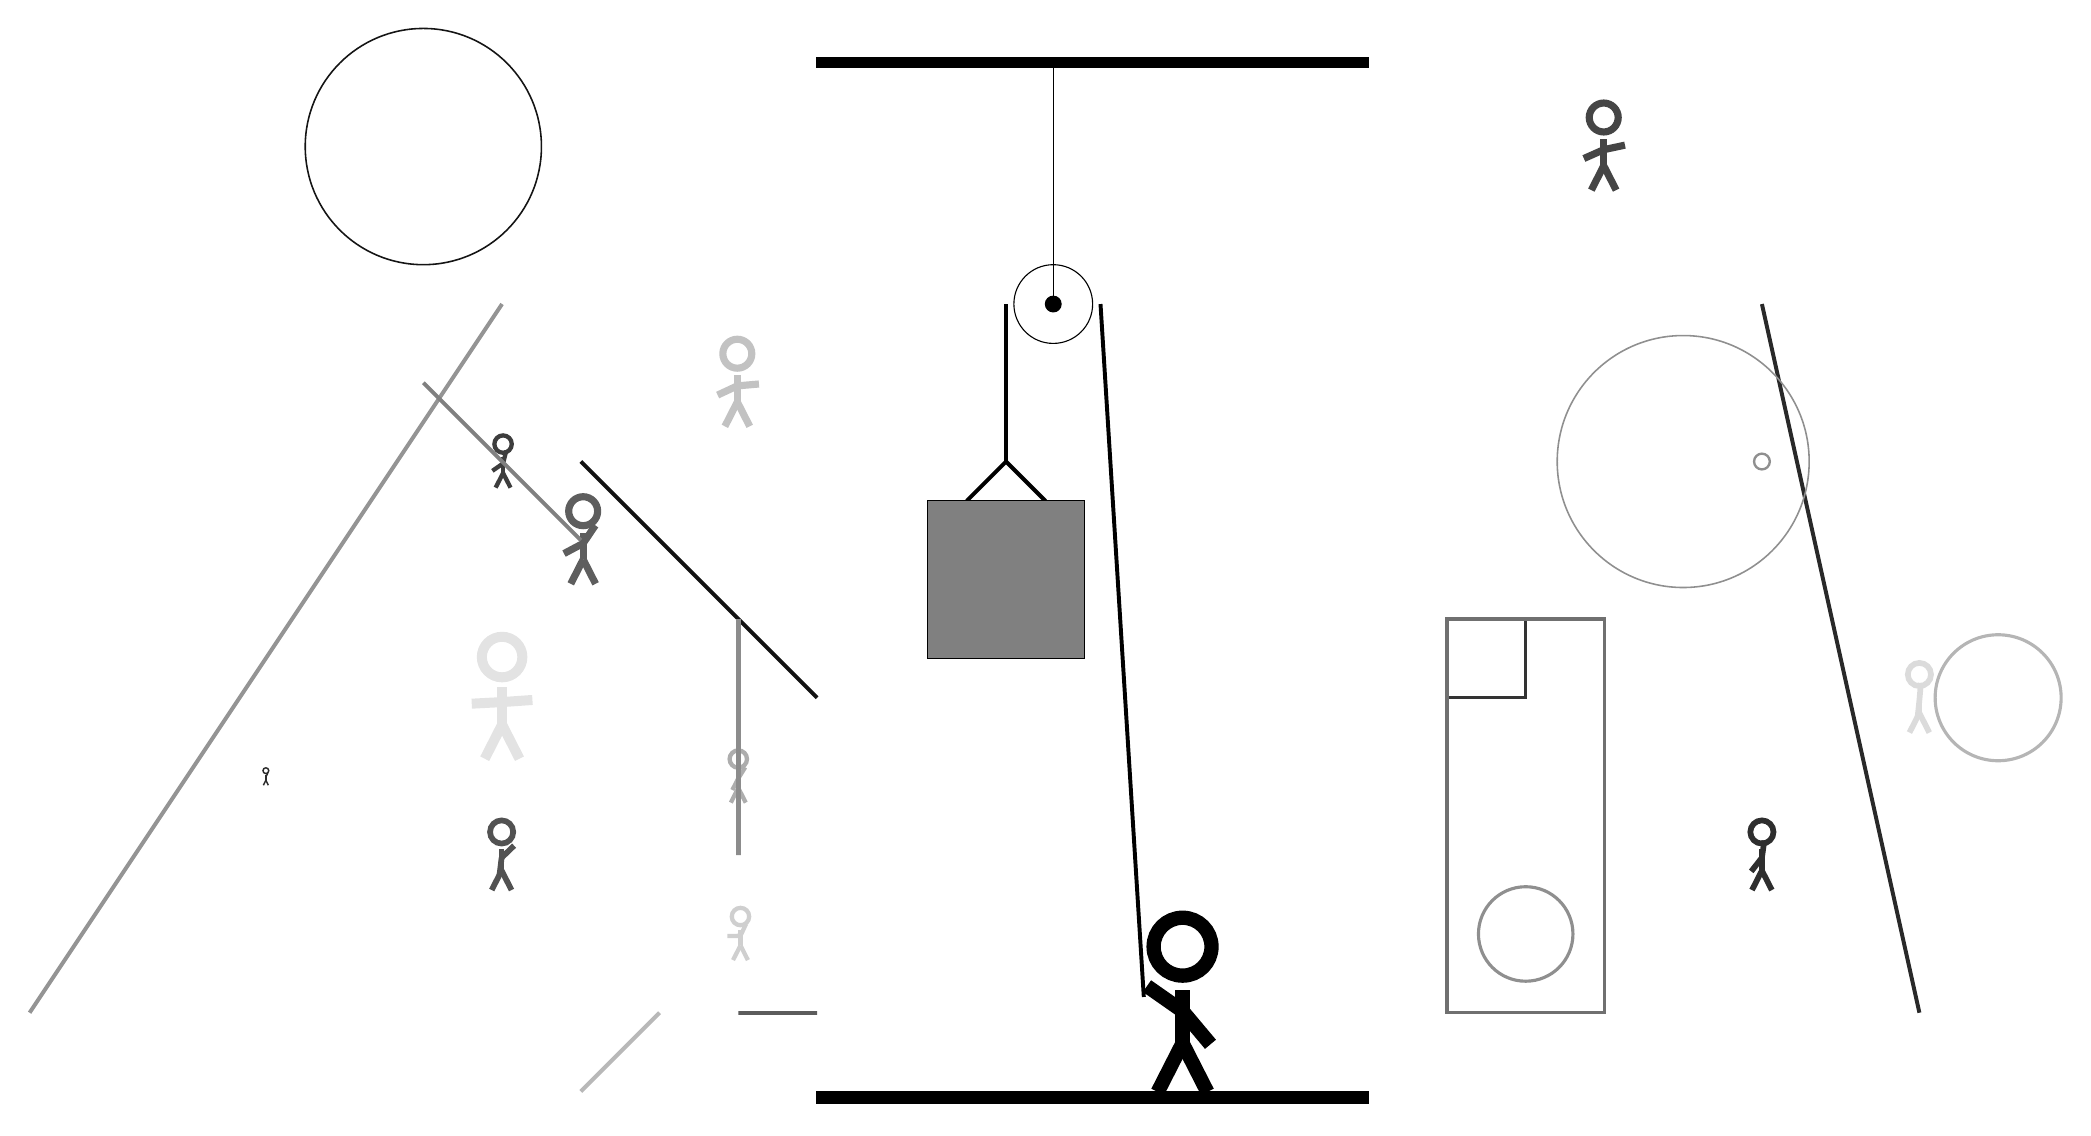
\begin{tikzpicture}
		%%%%% START %%%%%
		
		\draw[fill=black] (-2, 10) rectangle (5, 10.125);
		
		\draw (1, 7) circle (0.5);
		\draw[fill=black] (1, 7) circle (0.1);
		\draw (1, 10) -- (1, 7);
		
		\draw[line width=0.5mm] (-0.1, 4.5) -- (0.4, 5.0) -- (0.9, 4.5);
		\draw[fill=black!50] (-0.6, 4.5) rectangle (1.4, 2.5);
		
		\draw[line width=0.5mm] (0.4, 7) -- (0.4, 5.0);
		\centerarc[line width=0.5mm](1, 7)(0:180:0.6);
		\draw[line width=0.5mm](1.6, 7) -- (2.15, -1.8);
		
		\node[line width=0.4mm, color=black!82] at (10, 0) {\Strichmaxerl[4][52][82]};
		
		\node[line width=0.5mm, color=black!24] at (-3, 6) {\Strichmaxerl[5][25][5]};
		\draw[line width=0.4mm, color=black!80] (6, 2) rectangle (7, 3);
		\draw[line width=0.5mm, color=black!93](-2, 2) -- (-5, 5);
		\node[line width=0.2mm, color=black!11] at (-6, 2) {\Strichmaxerl[7][3][4]};
		\draw[line width=0.5mm, color=black!42](-6, 7) -- (-12, -2);
		
		\node[line width=0.5mm, color=black!73] at (8, 9) {\Strichmaxerl[5][24][12]};
		
		\draw [line width=0.4mm, color=black!29](13, 2) circle (0.8);
		\draw[line width=0.5mm, color=black!28](-5, -3) -- (-4, -2);
		
		\node[line width=0.3mm, color=black!83] at (-9, 1) {\Strichmaxerl[1][90][64]};
		\node[line width=0.3mm, color=black!63] at (-5, 4) {\Strichmaxerl[5][28][56]};
		
		\node[line width=0.3mm, color=black!32] at (-3, 1) {\Strichmaxerl[3][63][58]};
		\draw [line width=0.3mm, color=black!44](10, 5) circle (0.1);
		\draw[line width=0.4mm, color=black!56] (6, -2) rectangle (8, 3);
		\draw[line width=0.5mm, color=black!64] (-3, -2) rectangle (-2, -2);
		\node[line width=0.2mm, color=black!19] at (-3, -1) {\Strichmaxerl[3][1][65]};
		
		\draw[line width=0.6mm, color=black!45] (-3, 0) rectangle (-3, 3);
		
		\node[line width=0.3mm, color=black!76] at (-6, 5) {\Strichmaxerl[3][35][76]};
		\node[line width=0.3mm, color=black!68] at (-6, 0) {\Strichmaxerl[4][83][44]};
		\draw[line width=0.5mm, color=black!84](10, 7) -- (12, -2);
		\draw[line width=0.5mm, color=black!50](-5, 4) -- (-7, 6);
		
		\node[line width=0.7mm, color=black!14] at (12, 2) {\Strichmaxerl[4][84][85]};
		\draw [line width=0.4mm, color=black!44](7, -1) circle (0.6);
		\draw [line width=0.2mm, color=black!92](-7, 9) circle (1.5);
		\draw [line width=0.2mm, color=black!44](9, 5) circle (1.6);
		
		
		\node at (2.6, -1.9) {\Strichmaxerl[10][-35][-50]};
		
		\draw[fill=black] (-2, -3) rectangle (5, -3.15);
		
		%%%%% END %%%%%
	\end{tikzpicture}
\end{document}